\documentclass[12pt]{article}
\usepackage{ebgaramond}
\usepackage{apacite}
\usepackage[protrusion=true,expansion=true]{microtype} 
\usepackage{fullpage}
\usepackage{graphicx}
\setlength{\parskip}{0.5em}

\title{\textbf{Modeling Graphical Communication}}

\author{Judith Fan, Robert Hawkins, \& Justine Kao}

\begin{document}
\maketitle % Print the title section

\section{Motivation}

\subsection{Why graphical communication?}

Drawing is a powerful tool for communication --- with just a few strokes it is possible to convey the identity of a face \cite{bergmann2013impact} or express an intention to act \cite{Galantucci:2005uh}. Moreover, drawn images predate the historical record, are pervasive in human culture, and are often produced prolifically in childhood.

Examining graphical communication provides a window into how meaningful tokens emerge from individual experience and social interactions, especially when conventionalized carriers of meaning are not available (e.g., words). Over the long-term, integrating insights across studies of linguistic and graphical modes of communication may yield general principles that govern how people negotiate shared meanings.  

\subsection{How drawing influences object representations}

In ongoing work, Fan, Yamins, and Turk-Browne (in prep) are investigating the basis for the ability to communicate an idea by drawing, by evaluating the premise that our ability to recognize objects and produce recognizable drawings of objects are linked by a common internal substrate --- a generalized object representation. We found that a convolutional neural network whose architecture mirrors that of the ventral visual stream we was optimized to handle natural image variation in photographs \cite{Yamins:2014gia} was able to generalize to simple sketches of objects, without having to posit new specialized mechanisms. This suggests that the capacity for visual abstraction may be rooted in the functional architecture of the visual system.

Moreover, this result allows us to use this model as a tool to probe representational change: how does learning to draw objects influences the representation of object categories in the mind? Insofar as practice drawing allows one to learn the diagnostic features that better communicate the identity of an object (e.g., horse), they hypothesized that such practice might improve people's ability to make recognizable drawings of other, visually similar objects (e.g., sheep, cow). To test this, they designed a training paradigm in which participants repeatedly sketched some objects, while the model guessed the identity of the sketched object, providing trial-by-trial feedback. They found that repeatedly sketched objects were better recognized after training, while --- surprisingly --- sketches of unpracticed but similar objects worsened. These results show that visual production can reshape the representational space for objects in various ways: by differentiating trained objects and merging other nearby objects in the space.

\subsection{How do communicative interactions establish shared knowledge?}

How does social context constrain how ideas are expressed in drawings? That is, in addition to capturing physical properties of objects, successful drawings may depend on accurately representing the knowledge state of the viewer, coordinating on communicative intentions, and knowing what knowledge is shared in common ground. Such shared knowledge may derive from conventional knowledge, or may be established \textit{de novo} in the course of interactions between communication partners.

From \citeA{Brennan:1996ud} and others, we know that a individual's choice of label for an object is sensitive to the shared history of interactions with their interlocutor. Abstract objects are more accurately identified using descriptions written by the participant's own friends than by strangers \cite{fussell1989understanding}. Sometimes this results in the use of labels that might not be maximally efficient/distinctive in a given circumstance, but match the label previously used to refer to that same object (a ``conceptual pact'' about the object-label pairing). Furthermore, alignment in  phonemic, syntactic, and lexical choice is shown to correlate with performance on dyadic problem-solving tasks \cite{FusaroliBahrami2012}.

Additionally, prior work on graphical dialogue suggests that pairs of individuals who have interacted before tend to produce drawings that are more `abstract' and similar to one another than individuals who have had just as much experience with the drawing task, but previously interacted with other individuals \cite{Healey:2007vq}. Moreover, pairs that are able to `mutually-modify' each other's drawings in real time (as opposed to taking turns) also end up producing drawings with similar styles and are more abstract.  

Using a similar paradigm with word cues, \cite{Fay:2010jh} tracked pairs as they played several rounds of `Pictionary' with the same set of target items reappearing from round to round (e.g., `soap opera,' `parliament'). People initially produced detailed drawings that directly resembled their referents; however, over successive rounds, fewer strokes were necessary to convey the same meaning, and the drawings became progressively more iconic/symbolic \cite{Garrod:2007wk}. Drawings produced by members of the same pair to refer to a given target became more similar to one another, whereas drawings of a given target were highly variable across pairs, suggesting that the resulting conventions depend on the specific history of interactions between communication partners \cite{Fay:2010jh}.

Taken together, these studies provide converging evidence that rich social feedback plays a crucial role in refining graphical representations over repeated interactions; in the absence of this feedback, drawings can actually become more complex over time \cite{Garrod:2007wk,Hupet:1992ua}. Building on this prior work, the main goals of the present studies are: to systematically document major behavioral effects in this domain through a series of interrelated experiments, and to build a quantitatively predictive model that captures how social interactions shape the representational content of communicative drawings, thereby explaining how such experiences can lead to both efficient and expressive communication \cite{Kirby:2015gi}. 

\section{Proposal}

\subsection{How does interaction history guide graphical communication?}

How do two people who interact repeatedly negotiate shared graphical conventions for expressing their ideas? Moreover, does sharing a history of interactions help when needing to express some new idea (or interpret a new meaning expressed by a familiar conversation partner)? 

To accomplish this, we plan to develop a graphical-dialogue paradigm in which one participant (Artist) has the goal of producing drawings of objects that the other participant (Viewer) will be able to identify. To investigate the importance of interaction history, we will manipulate how much and what kinds of objects they practice drawing/identifying before they are tested on a set of novel objects.

\subsection{Stimuli}

Objects will be sampled from a set of four real-world object categories defined at the basic level: dogs, birds, cars, and airplanes. Each category will contain eight exemplars. 

Images of these objects will serve as cues in the drawing task, as well as alternatives in the identification task. These images will be rendered from 3D mesh models, permitting fine control over low-level visual properties of these images, including size, viewpoint, and illumination. 

\begin{figure}[hbtp]
\begin{center}
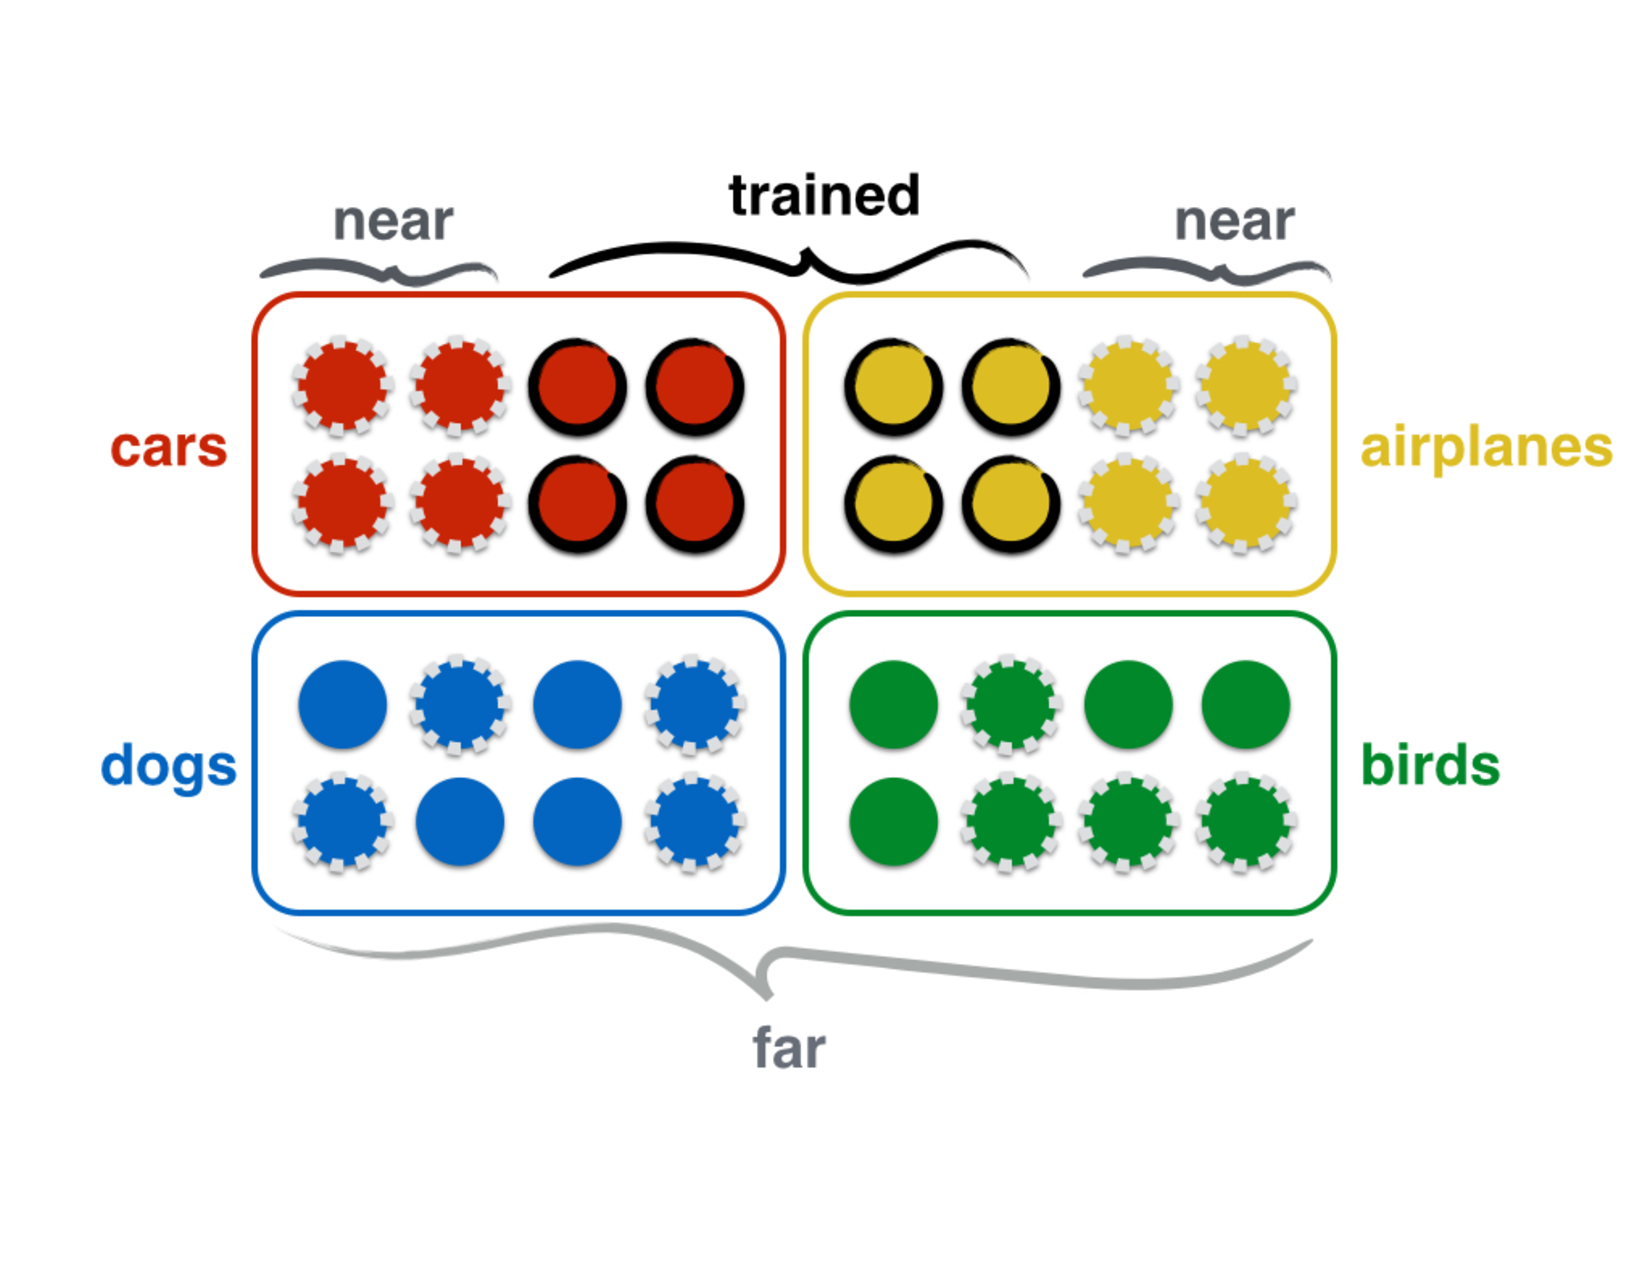
\includegraphics[width=80mm]{figures/design.pdf}
\end{center}
\end{figure}
\vspace{-10mm}

\subsection{General Procedure}

Adopting a similar approach to Fan, Yamins, and Turk-Browne (in prep), we plan to employ an experimental design that probes generalization by contrasting test performance on untrained objects that belong to the same category as trained objects with performance on untrained objects that belong to a different category. 

For each session, we will recruit two naive participants. During an initial learning phase, each participant will take turns as Artist and Viewer, alternating roles on each trial. They will practice on the same subset of objects (4 of 8) sampled from half of the categories (2 of 4). Each participant will draw each object twice, resulting in 64 total learning trials, comprising 16 drawing trials and 16 guessing trials for each participant. These trials may be blocked by category, such that all the trials in the same block involve objects from the same category (4 blocks, 2 per category). 

On each trial of this practice phase, the Artist will be cued with an image of one of these objects (target) and prompted to produce a quick sketch of it (<=30s). This sketch will then be revealed to the Viewer, whereupon he/she will guess which object the sketch corresponds to by selecting among all 8 alternatives from the target category. These alternatives will be displayed as images depicting each of the trained objects from identical viewpoints. After the Viewer makes a guess, the pair will receive feedback indicating whether the choice was correct or not; if incorrect, the Viewer will be shown which object was the target. 

The test phase will immediately follow the practice phase. During this phase, participants will attempt to communicate the remaining objects in the trained categories (8 total, 4 from each category, `Near'), as well as a subset of objects (4 of 8) sampled from the held-out categories (2 of 4, `Far'). At test, participants will not be interacting on a trial-by-trial basis. Instead, each will first complete an Artist block in which they draw a series of novel objects without feedback, then a Viewer block in which they identify the object in the test sketches produced by their communication partner. Each participant will draw every object once, resulting in 16 drawing trials and 16 guessing trials. 

\subsection{General Predictions}

\subsubsection{Training}

As both participants encounter each object in the Artist and Viewer roles once before doing so a second time in the practice phase, we can analyze the first and second halves of the practice phase separately in order to examine the consequences of the first complete graphical exchange. If this exchange leads to greater coordination of graphical tokens used to evoke objects, we would predict higher identification accuracy, as well as higher feature similarity between their drawings (based on top-layer model output from the CNN described in \citeNP{Yamins:2014gia}) on the second repetition of the practice phase relative to the first. The degree of improvement could be contrasted with a non-interactive control condition in which participants first drew all trained objects twice, then made guesses about their partner's drawings after the fact. 

\subsubsection{Generalization}

Does interacting extensively with an individual have more general consequences, affecting how other, related ideas are expressed (and understood)? If learning how to make drawings that convey the identity of objects belonging to the same category (e.g., poodle, dalmatian) depends on coordinating graphical conventions for capturing their distinguishing features within this category, the members of this pair may be able to generalize to other members of the same category (e.g., schnauzer). If true, generalization may still occur for objects from untrained categories, but to a much lesser extent. The degree of generalization observed in this case could be contrasted with a switched-pair control condition in which participants trained with one partner, but performed the generalization test with a member of a different pair who had trained on the same objects. 

\subsection{Specific Manipulations}

There are several variations on the basic procedure outlined above that would allow us to pose more specific questions about how interaction history influences graphical communication.

\begin{figure}[hbtp]
\begin{center}
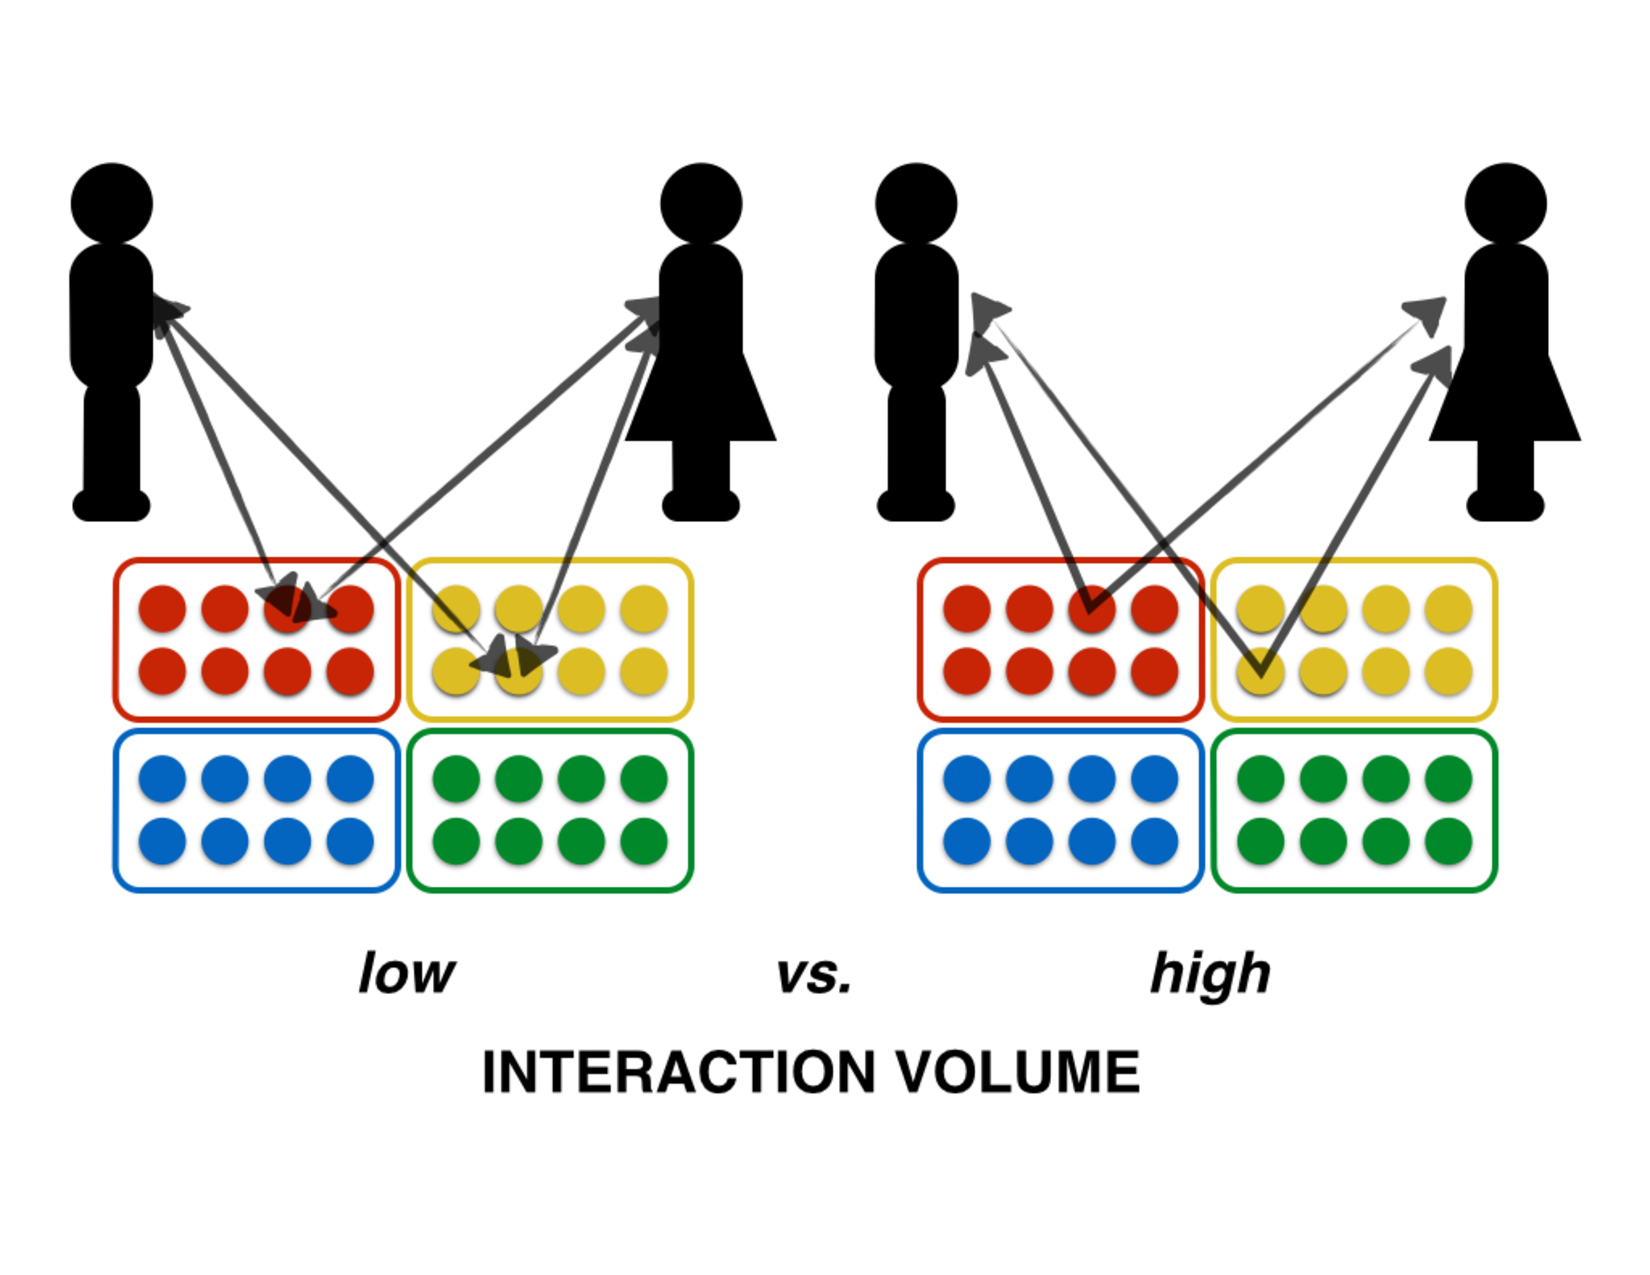
\includegraphics[width=80mm]{figures/interaction_volume.pdf}
\end{center}
\end{figure}
\vspace{-5mm}

\subsubsection{Interaction volume} How does the sheer number of interactions two people have influence how well they are able to generalize to communicating new concepts? Insofar as interaction history meaningfully influences how people communicate, people with the same amount of experience drawing and guessing but who did not previously interact with each other may be at a disadvantage. 

To test this, we could compare test performance between pairs trained in the manner described above with that of a control group in which pairs do not interact prior to being tested. On drawing-practice trials in this Control condition, participants practice drawing the same objects the same number of times as above, but receive either no feedback or only feedback based on model-classifier output. On guessing-practice trials, these control participants would be prompted to label drawings produced by randomly sampled other participants from other sessions. 

\subsubsection{Conceptual overlap} Oftentimes two people enter into a conversation wishing to express different ideas, but have an interest in understanding what the other person means. How does this circumstance initially affect how effectively they communicate, and how do they go about bridging across these differences? 

In the general procedure above, both participants receive equal amounts of experience learning to express the same set of concepts, as well as interpret drawings conveying them. Thus, this baseline case represents maximal overlap in communicative goals and prior experience. In a close variant of this that reduces overlap between their direct experiences, one participant would be assigned all (four) trained items from one category, and the other participant the other category. He/she would only practice drawing objects from one category, and only practice interpreting drawings made by their partner of objects from the other category. For the pair as a whole, this condition is identical to the baseline condition, in that they are collectively exposed to the same objects the same number of times in each task modality, except that each participant's experiences in each task are biased towards one category. How does this specialization affect how well each participant is able to adapt their drawings to be more recognizable to their communication partner during the practice phase, and what are the consequences for generalization in the test phase?

\begin{figure}[hbtp]
\begin{center}
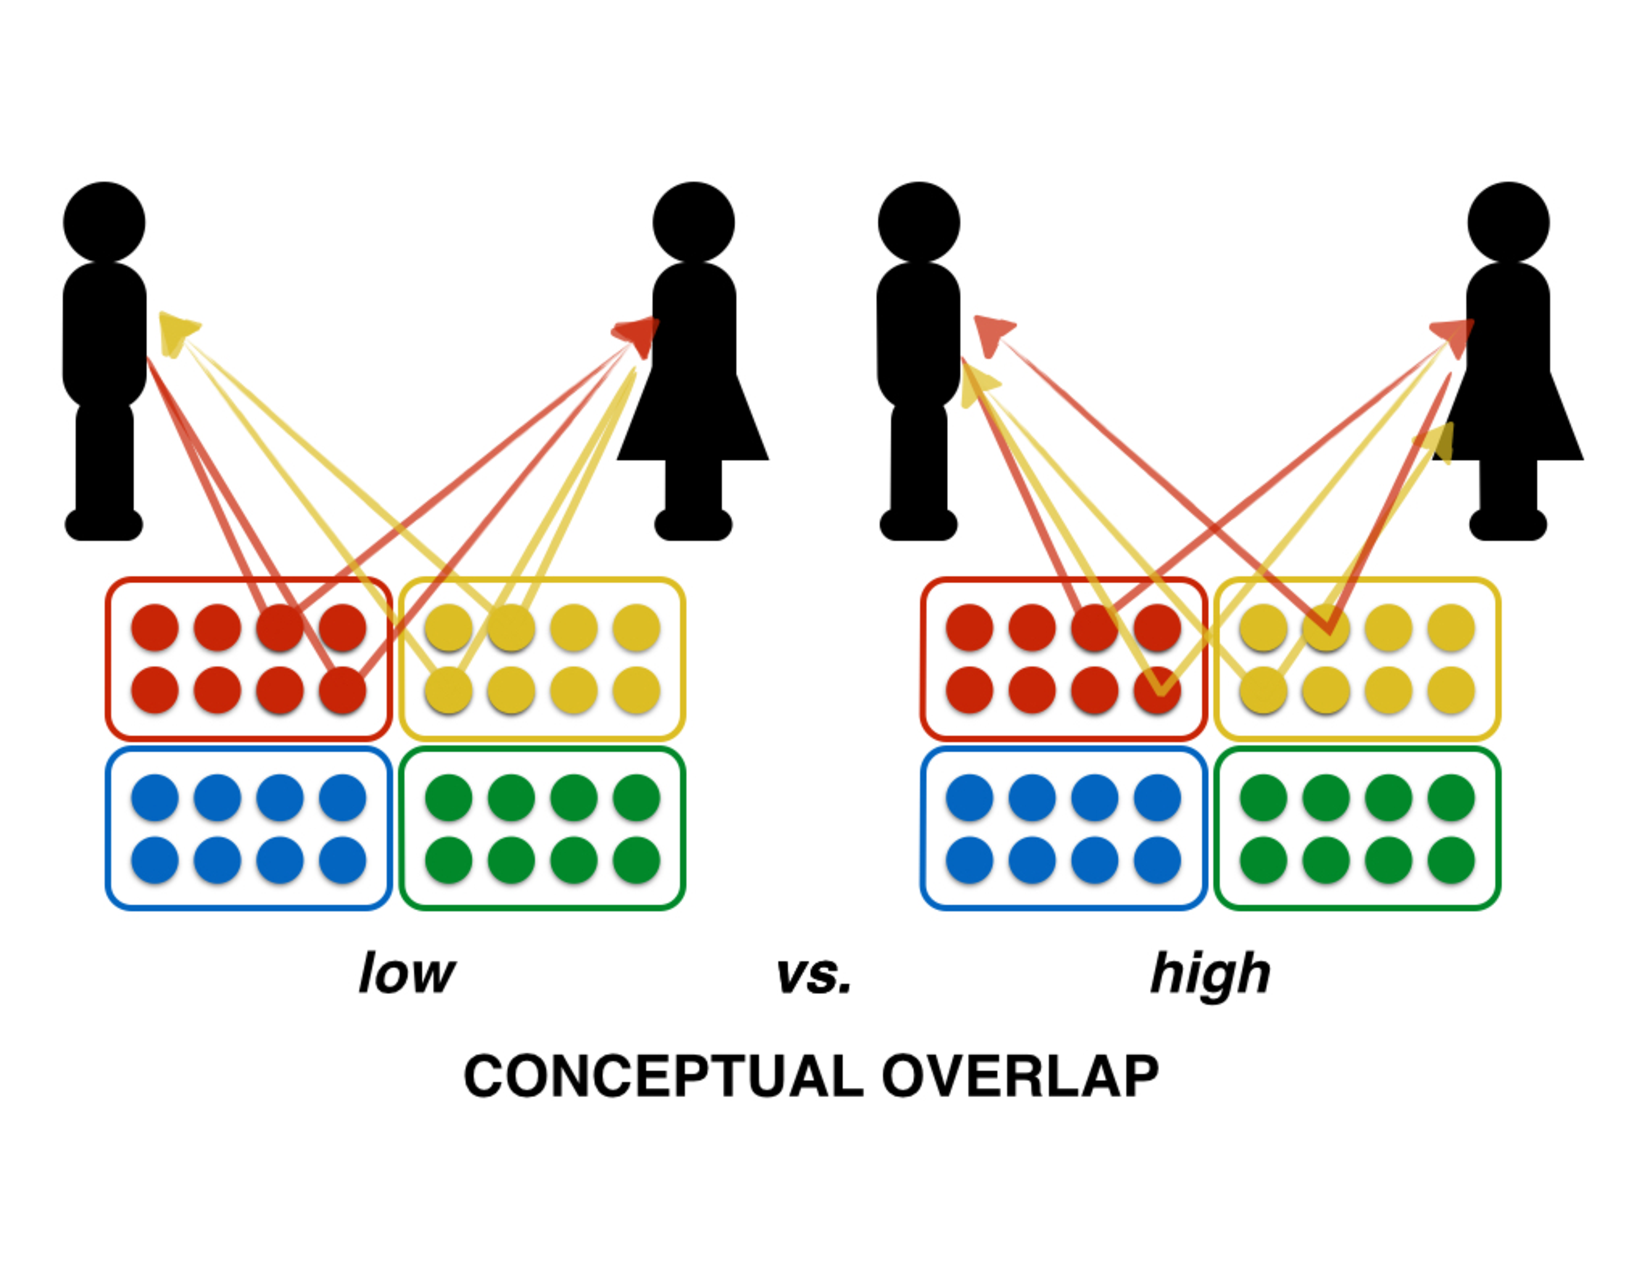
\includegraphics[width=80mm]{figures/conceptual_overlap.pdf}
\end{center}
\end{figure}
\vspace{-5mm}

\subsubsection{Knowledge asymmetries} In many real-world scenarios, there are often knowledge asymmetries between communication partners (e.g. that between a teacher and a student). Such asymmetries can sometimes be a source of confusion, when the relatively more-knowledgeable individual uses terms or conventions that the less-knowledgeable individual is unfamiliar with. What kinds of strategies can the pair adopt in order to cope with such asymmetries, and still communicate effectively? 

In our paradigm, inducing an asymmetry in experience could be accomplished by pre-training one member of the pair on several more objects prior to beginning to interact with the other participant (similar to `director' in \citeNP{Wu:2007tz}). In order to minimize the risk of interference with subsequent social feedback, this pre-training could be performed without external feedback. Insofar as this pre-training promoted greater abstraction in this participant's drawings, this might initially hinder communication with a naive Viewer, who may not share the same visual abstractions. In the absence of explicit disclosure from the experimenters that there was an asymmetry in training, how do the dynamics of interaction under these conditions compare with those of the symmetric baseline condition? Does this pre-training make it easier (or more difficult) to interpret the drawings of the naive participant? Is it more likely that the pair converges on conventions proposed by the pre-trained participant, or the naive one? 

\begin{figure}[hbtp]
\begin{center}
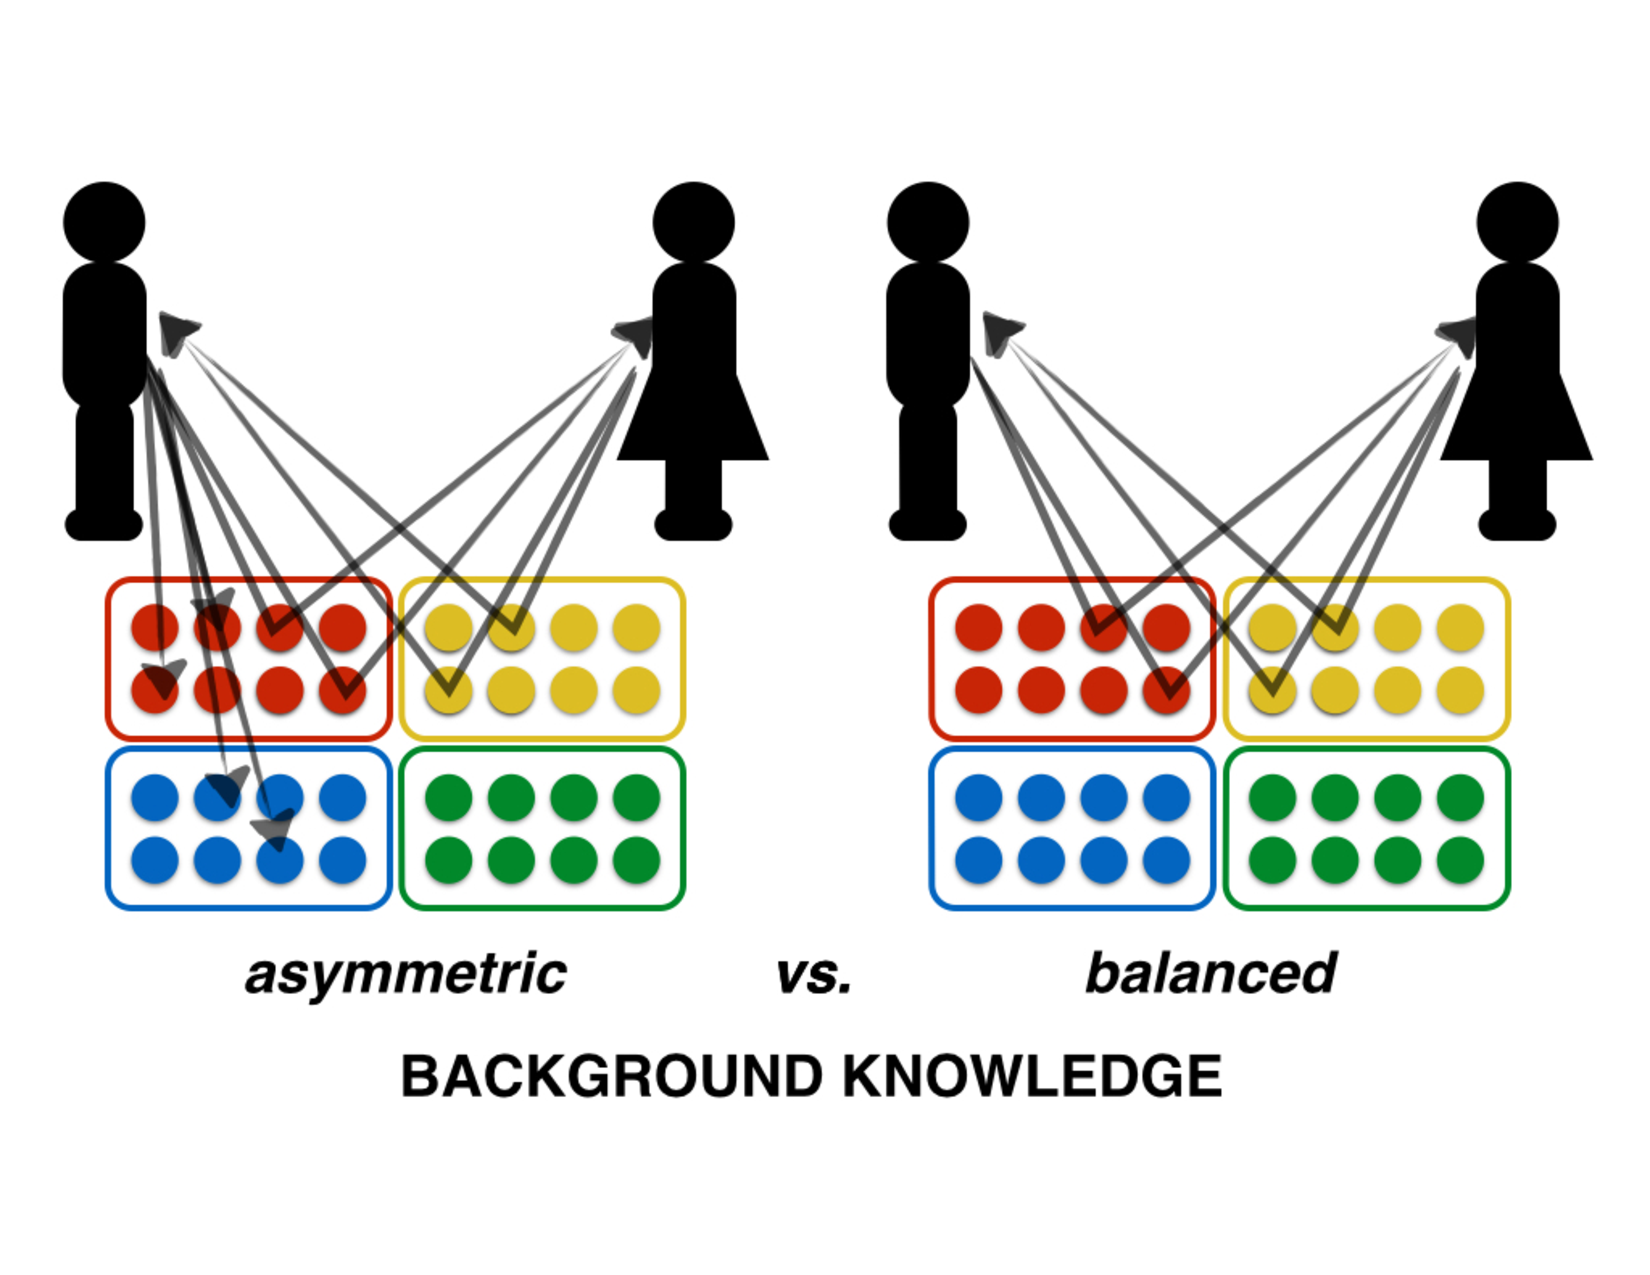
\includegraphics[width=80mm]{figures/background_knowledge.pdf}
\end{center}
\end{figure}
\vspace{-5mm}

\subsubsection{Pragmatic considerations} How does an Artist's knowledge of the Viewer's belief state influence how they draw? For example, if the Artist knew ahead of time the space of alternatives that the Viewer was considering (operationalized as options presented in the forced-choice task), how would this affect which features he/she included? In the design described above, the list of alternatives presented are always exhaustive directories of the exemplars belonging to a single basic-level category. This might promote search for the feature(s) that were most diagnostic of the specific identity of the target relative to the other exemplars within the same category. On the other hand, if the list of alternatives included objects belonging to different categories, this might promote the selection of alternate features, perhaps those diagnostic of the basic-level category containing the target, but not uniquely possesed by it. 

\begin{figure}[hbtp]
\begin{center}
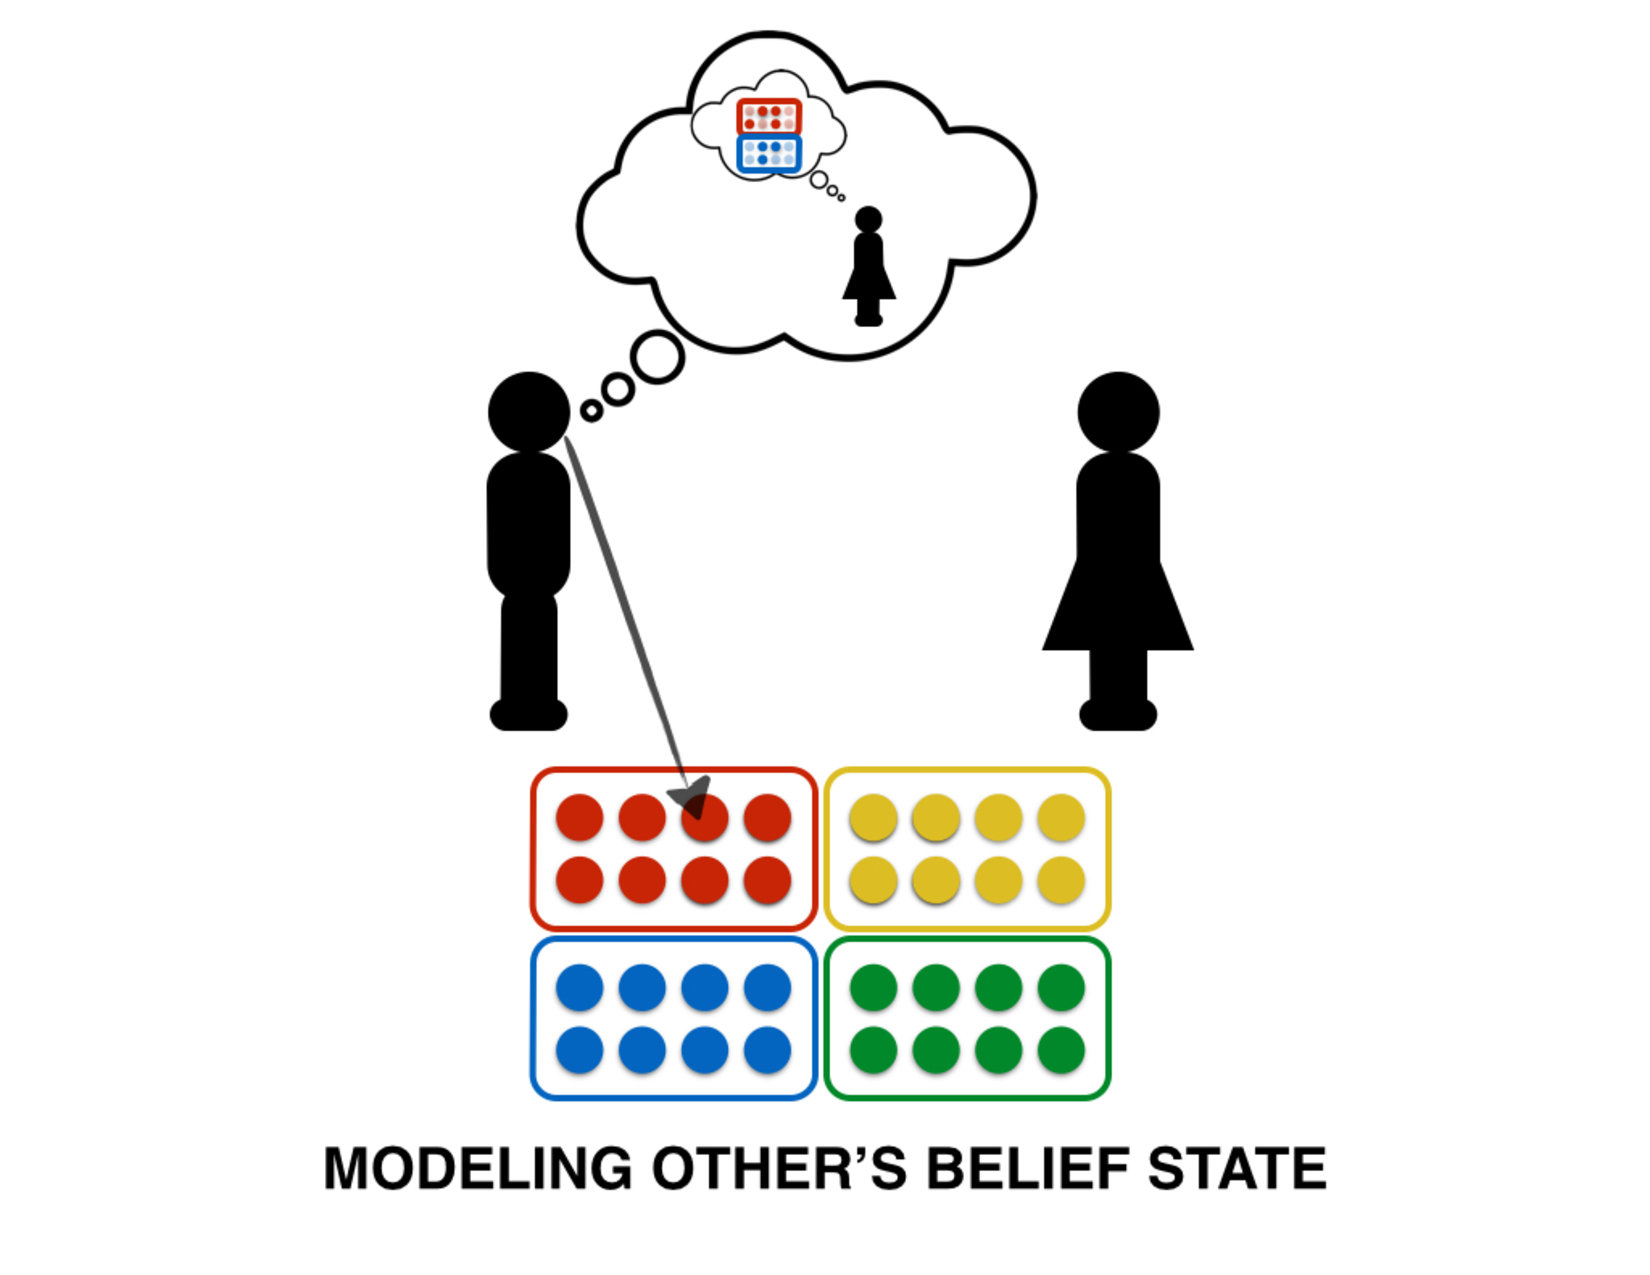
\includegraphics[width=80mm]{figures/pragmatic_considerations.pdf}
\end{center}
\end{figure}
\vspace{-5mm}

Conversely, how does a Viewer's knowledge of the Artist's goals influence how they construe a drawing? For example, a Viewer who learns that the Artist is penalized for the amount of `ink' used during drawing may discount the presence or absence of dense texture fills in their drawing, even if this is otherwise a highly diagnostic feature of the target object. There are other ways to manipulate the Viewer's expectations about the Artist's intentions, given the drawing in front of them, as well. One may be to compromise the quality of the perceptual information the Artist has about the target (e.g., an uninformative viewpoint, or blurred image) and pass this information along to the Viewer.


\subsection{A future direction: emergence of novel graphical conventions}

In some cases, verbal and visual conventions for referring to objects may not be well established (e.g., music drawing task from \citeNP{Healey:2007vq}), or not available at all (cf. coordination game in \citeNP{Galantucci:2005uh}). For instance, auditory textures \cite{McDermott:2013ky} lack the rhythmic and pitch information that are captured in standard musical notation, and may be hard to describe. Thus, someone who wants to visually convey which auditory texture they are listening to must innovate a graphical scheme for capturing its identifying physical features. While the initial selection of encoding schemes may be highly underdetermined, how do repeated interactions between communication partners induce convergence upon a consistent way of referring to these shared experiences?

\bibliographystyle{apacite}
\setlength{\bibleftmargin}{.125in}
\setlength{\bibindent}{-\bibleftmargin}
\bibliography{references.bib}

\end{document}
